\chapter{Chapter 1 appendix}
\section{Mathematical description of simple labelling flux}
\label{chap1_app:flux}
A common goal of stable isotope tracing is the measurement of flux through a pathway.
This requires a mathematical description of the system with a set of associated assumptions.
Here such description is provided for a very simple system describing a single metabolic reaction.

The system is illustrated in figure \ref{fig:app_ch1:tracing_diagram} and contains one or more cells with total volume $V(t)$, proliferating with growth rate $g$ and two metabolites with the concentrations $A$ and $B$.
$A_{out}$ is situated outside of the cell, upon transport into the cell at a rate $r_{in}$, it becomes available for conversion into $B$ at a rate $r_{AB}$, whereafter it is exported outside the cell at a rate $r_{out}$.
These metabolites are either labelled ($A^L$) or unlabelled ($A^U$) and sum describes the total concentration i.e. $A = A^L + A^U$.

For this system a number of assumptions are made:
1) cell proliferation is constant,
2) the concentrations $A_{out}$, $A$ and $B$ are constant,
3) all reactions (indicated by arrows) are irreversible,
4) the labelling fraction of $A$ is constant and the same both inside and outside.

The objective is to determine the flux from $A$ to $B$ ($F_{AB} = A\ r_{AB}$) in order to describe $B^L$ and $B^U$ over time.

\begin{figure}[ht]
    \centering
    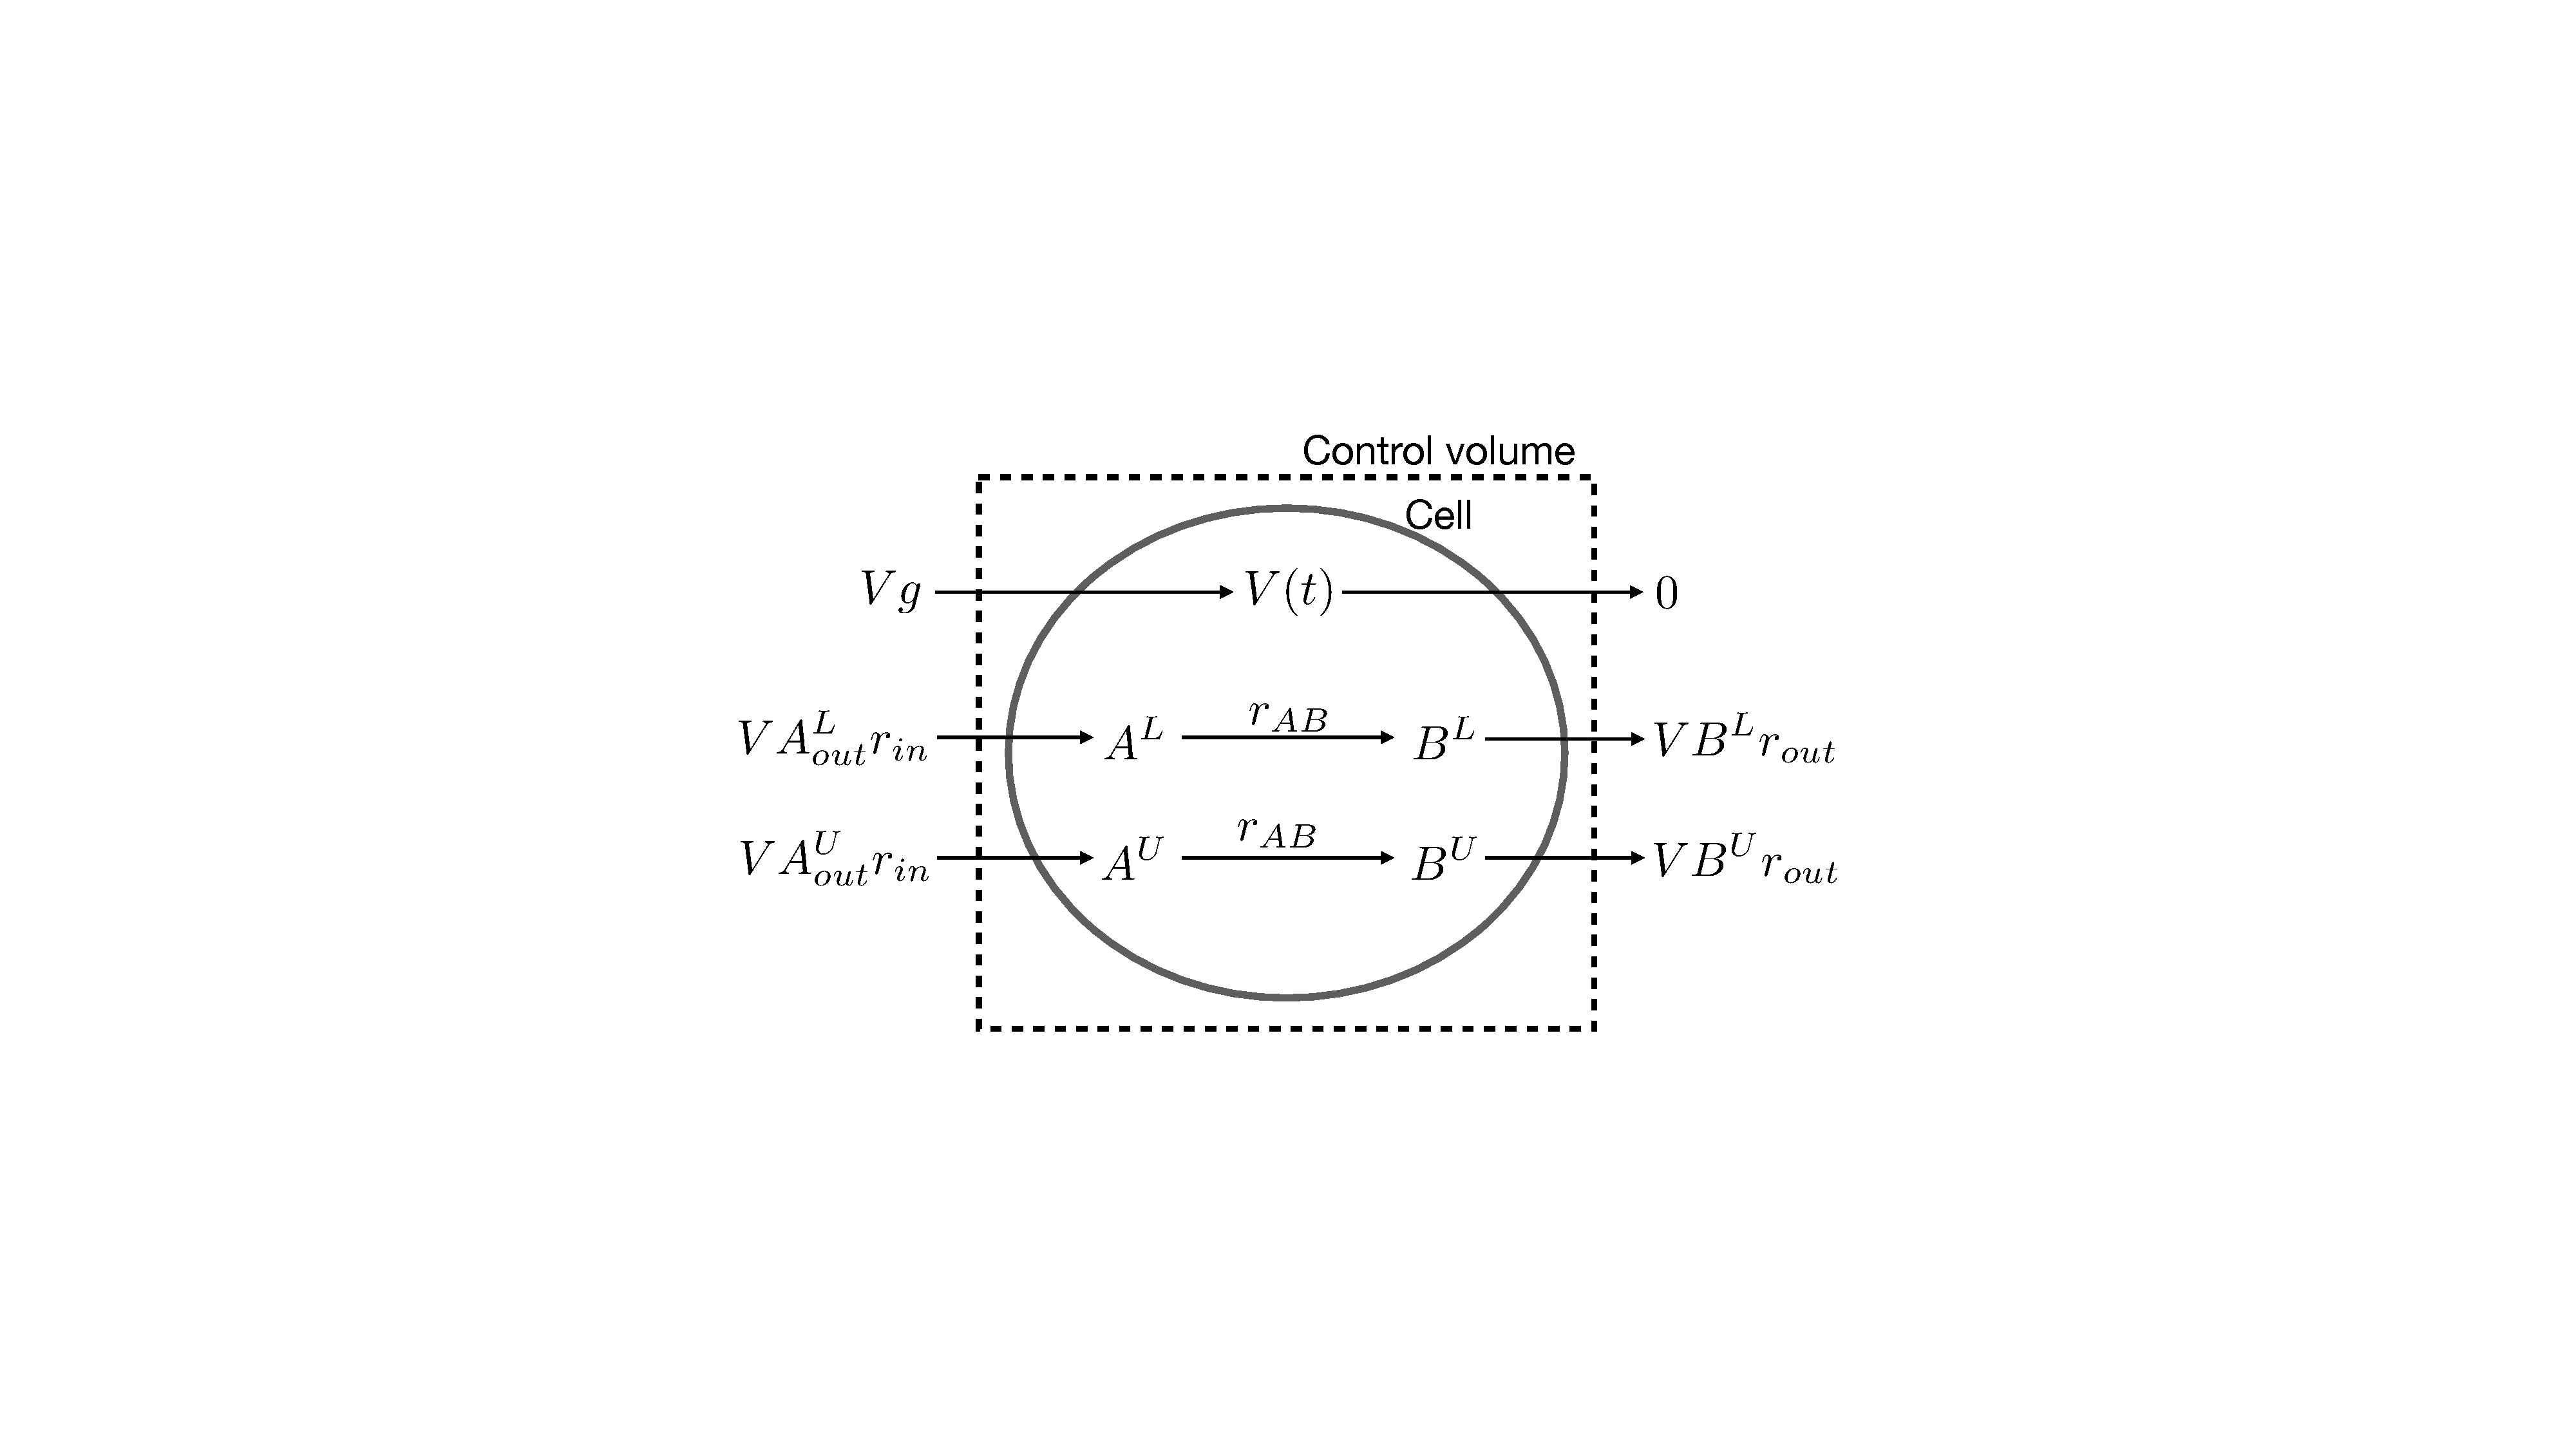
\includegraphics[width=0.7\textwidth]{figures/chap1/app/tracing_diagram.pdf}
    \caption[Mass balance diagram for metabolite labelling.]{
    Mass balance diagram for labelling of metabolite $B$.
    See text for details.
    }
    \label{fig:app_ch1:tracing_diagram}
\end{figure}


To deal with labelled and unlabelled metabolites the labelling fraction, which is constant for $A$, is introduced:
\begin{equation}
    \alpha = \frac{A^L}{A^L +A^U} = \frac{A^L}{A} \Longrightarrow A^L = \alpha A
\label{eq:app_ch1:alpha}
\end{equation}

For $B$ the labelling fraction changes over time:
\begin{equation}
    \beta(t) = \frac{B^L}{B^L +B^U} = \frac{B^L}{B} \Longrightarrow B^L = \beta B
\label{eq:app_ch1:beta}
\end{equation}

For the cell volume we know that it follows standard exponential growth with initial condition $V(0) = V_0$ such that:
\begin{equation}
    V(t) = V_0 e^{g t}
\label{eq:app_ch1:cell_vol}
\end{equation}
This could also be derived from the mass balance, assuming constant cell density.

Now, applying mass balance of the control volume (IN - OUT = ACCUMULATED) on $A^L$ over a time difference of $\Delta t$:
\begin{equation}
    V \alpha A_{out}\ r_{in} \Delta t - V \alpha A\ r_{AB} \Delta t = (V \alpha A)(t + \Delta t) - (V \alpha A)(t)
\label{eq:app_ch1:A_balance}
\end{equation}
Rearrange:
\begin{equation}
    \frac{(V \alpha A)(t + \Delta t) - (V \alpha A)(t)}{\Delta t} = V \alpha A_{out}\ r_{in} - V \alpha A\ r_{AB}
\label{eq:app_ch1:A_dq1}
\end{equation}
Let $\Delta t \rightarrow 0$ and the differential quotient emerge:
\begin{equation}
    \frac{d}{dt} (V \alpha A) = V \alpha A_{out}\ r_{in} - V \alpha A\ r_{AB} = \alpha A \frac{d V}{dt} + V \alpha \frac{dA}{dt}
\label{eq:app_ch1:A_dq2}
\end{equation}
From assumption 4) above it is known that $\frac{dA}{dt} = 0$, also from the volume equation (equation \ref{eq:app_ch1:cell_vol}) it is observed that $\frac{dV}{dt} = V g$:
\begin{equation}
    \alpha A V\ g = V \alpha A_{out}\ r_{in} - V \alpha A\ r_{AB} \Longrightarrow A_{out}\ r_{in} = A\ r_{AB} + A\ g
\label{eq:app_ch1:A_dq2s}
\end{equation}
This can be interpreted as influx ($F_{in}$) is equal to consumption flux to B ($F_{AB}$) plus flux to maintain constant concentration $A$ while cells are replicating ($F^A_{rep}$):
\begin{equation}
    A_{out}\ r_{in} = A\ r_{AB} + A\ g \Longrightarrow F_{in} = F_{AB} + F^A_{rep}
\label{eq:app_ch1:A_flux}
\end{equation}


Similarly, applying mass balance on $B^L$:
\begin{equation}
    V \alpha A\ r_{AB} \Delta t - V \beta B\ r_{out} \Delta t = (V \beta B)(t + \Delta t) - (V \beta B)(t)
\label{eq:app_ch1:B_balance}
\end{equation}
\begin{equation}
    \frac{(V \beta B)(t + \Delta t) - (V \beta B)(t)}{\Delta t} = V \alpha A\ r_{AB} - V \beta B\ r_{out}
\label{eq:app_ch1:B_dq1}
\end{equation}
\begin{equation}
    \frac{d}{dt} (V \beta B) = V \alpha A\ r_{AB} - V \beta B\ r_{out} = \beta B \frac{d V}{dt} + V B \frac{d\beta}{dt}
\label{eq:app_ch1:B_dq2}
\end{equation}
\begin{equation}
    \beta B\ g + B \frac{d\beta}{dt} = \alpha A\ r_{AB} - \beta B\ r_{out}
\label{eq:app_ch1:B_dq2s}
\end{equation}
The flux from $A$ to $B$  has already been defined as $F_{AB} = A\ r_{AB}$, also let $F_{out} = B\ r_{out}$ and $F^B_{rep} = B\ g$:
\begin{equation}
     \beta F^B_{rep} + B \frac{d\beta}{dt} = \alpha F_{AB} - \beta F_{out}
\label{eq:app_ch1:B_dq2s2}
\end{equation}
Rearrange:
\begin{equation}
     B \frac{d\beta}{dt} = \alpha F_{AB} - \beta (F_{out} - F^B_{rep})
\label{eq:app_ch1:B_dq2s3}
\end{equation}
Observe, similar to equation \ref{eq:app_ch1:A_flux} that $F_{out} = F_{AB} + F^B_{rep}$ and insert:
\begin{equation}
     \frac{d\beta}{dt} = (\alpha - \beta) \frac{F_{AB}}{B}
\label{eq:app_ch1:B_dq2s4}
\end{equation}
By integration the labelling fraction of $B$ is found:
\begin{equation}
     \beta(t) = \alpha + C e^{-\frac{F_{AB}}{B} t}
\label{eq:app_ch1:B_t}
\end{equation}
In most cases there will be no labelling of $B$ at time zero i.e. an initial condition of $\beta(t) = 0$, resulting in integration constant $C = -\alpha$:
\begin{equation}
     \beta(t) = \alpha - \alpha e^{-\frac{F_{AB}}{B} t}
\label{eq:app_ch1:B_t_IC}
\end{equation}


A useful descriptor is the time to half-max labelling, or more generally the time ($t_{\lambda}$) to fraction-of-max ($\lambda \in [0, 1]$) labelling:
\begin{equation}
     \lambda = \frac{\beta(t_{\lambda})}{\beta(\infty)} = \frac{\alpha - \alpha e^{-\frac{F_{AB}}{B} t_{\lambda}}}{\alpha}
\label{eq:app_ch1:B_hl}
\end{equation}
Isolating the time:
\begin{equation}
     t_{\lambda} = \frac{B}{F_{AB}} \ln\left( \frac{1}{1 - \lambda} \right)
\label{eq:app_ch1:B_hl2}
\end{equation}

Finally as an example, glutamine to glutamate synthesis flux is estimate to 30 mM/h and the intracellular pool of glutamate is estimate to a concentration of 5 mM.
How long does it take to reach 95\% of max labelling from glutamine?
\begin{equation}
     \frac{5\ mM}{30\ mM/h} \ln\left( \frac{1}{1 - 0.95} \right) \approx 0.5\ h
\label{eq:app_ch1:B_glu}
\end{equation}





\newpage
\section{Pig serum nucleoside/base concentrations}
\label{chap1_app:serum}
\begin{figure}[ht]
    \centering
    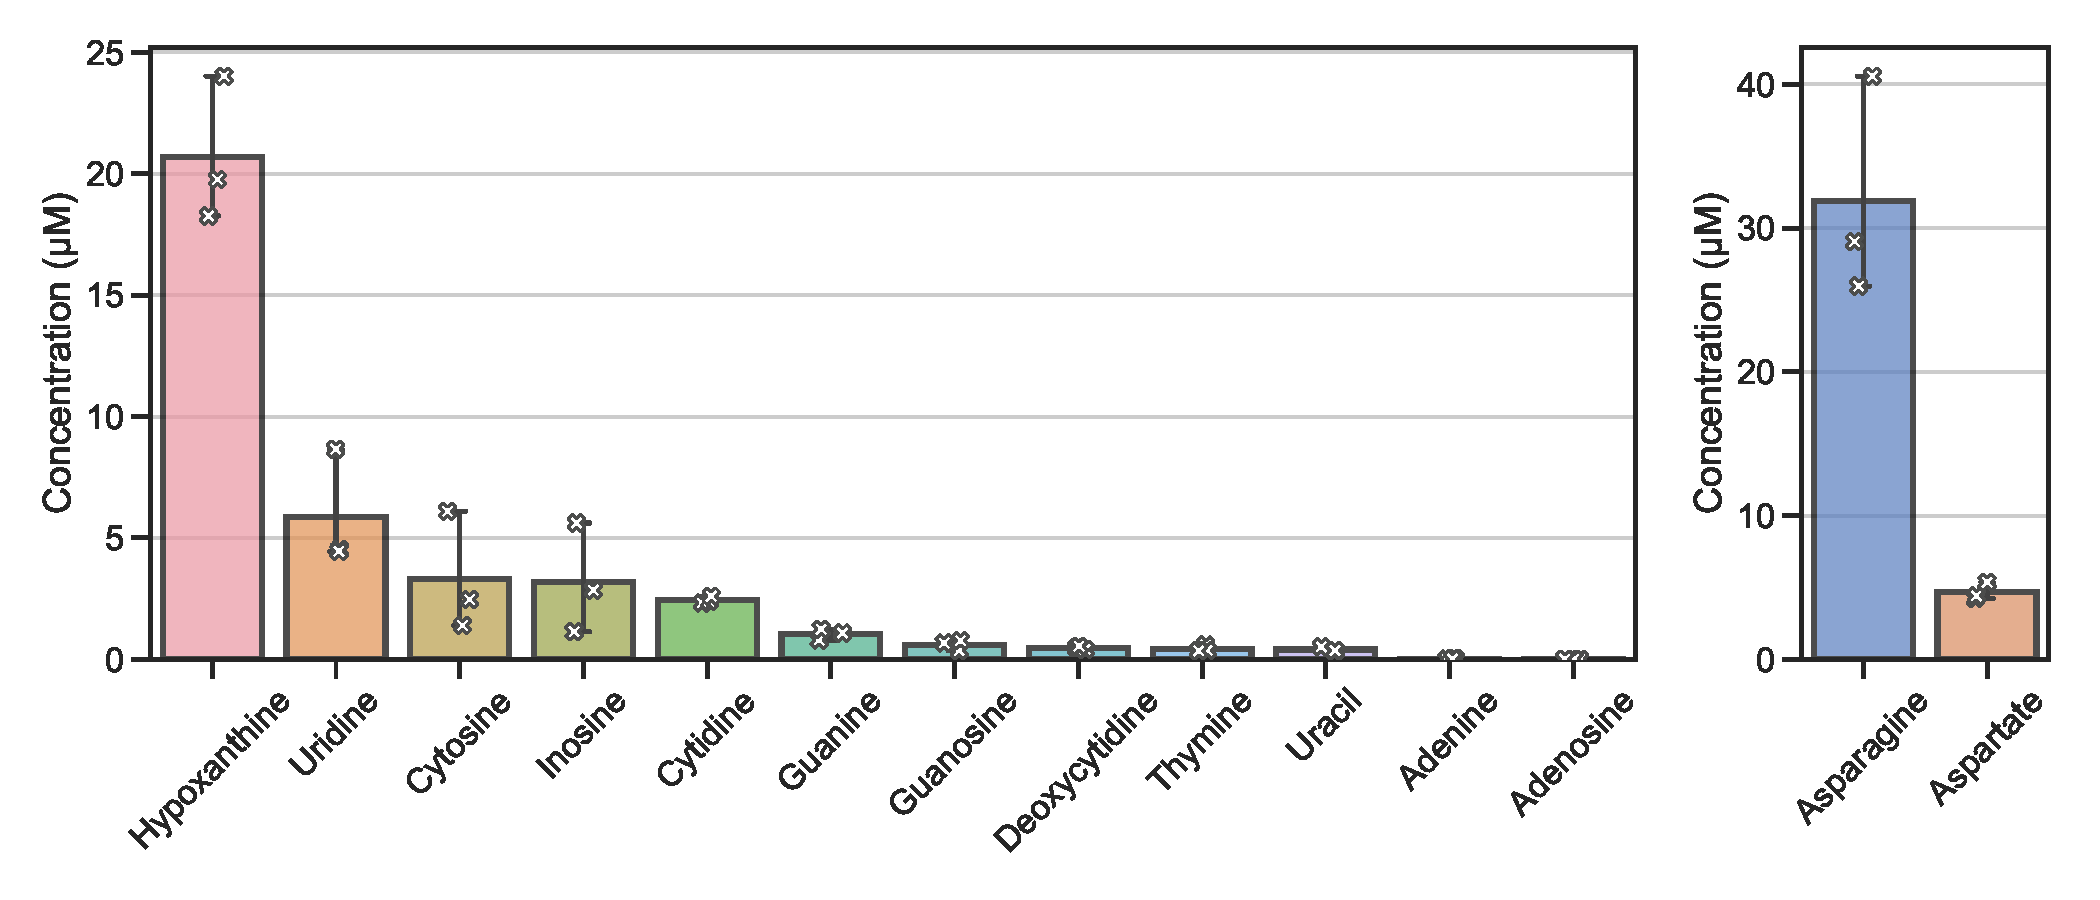
\includegraphics[width=0.85\textwidth]{figures/chap1/app/pig_nucl_conc.pdf}
    \caption[Pig serum nucleoside/base concentrations.]{
    Pig serum nucleoside/base concentrations determined using LCMS isotope dilution.
    }
    \label{fig:app_ch1:pig_nucl_conc}
\end{figure}

\newpage
\section{Fumarate regeneration to aspartate}
\label{chap1_app:fumarate_NAD}
\begin{figure}[ht]
    \centering
    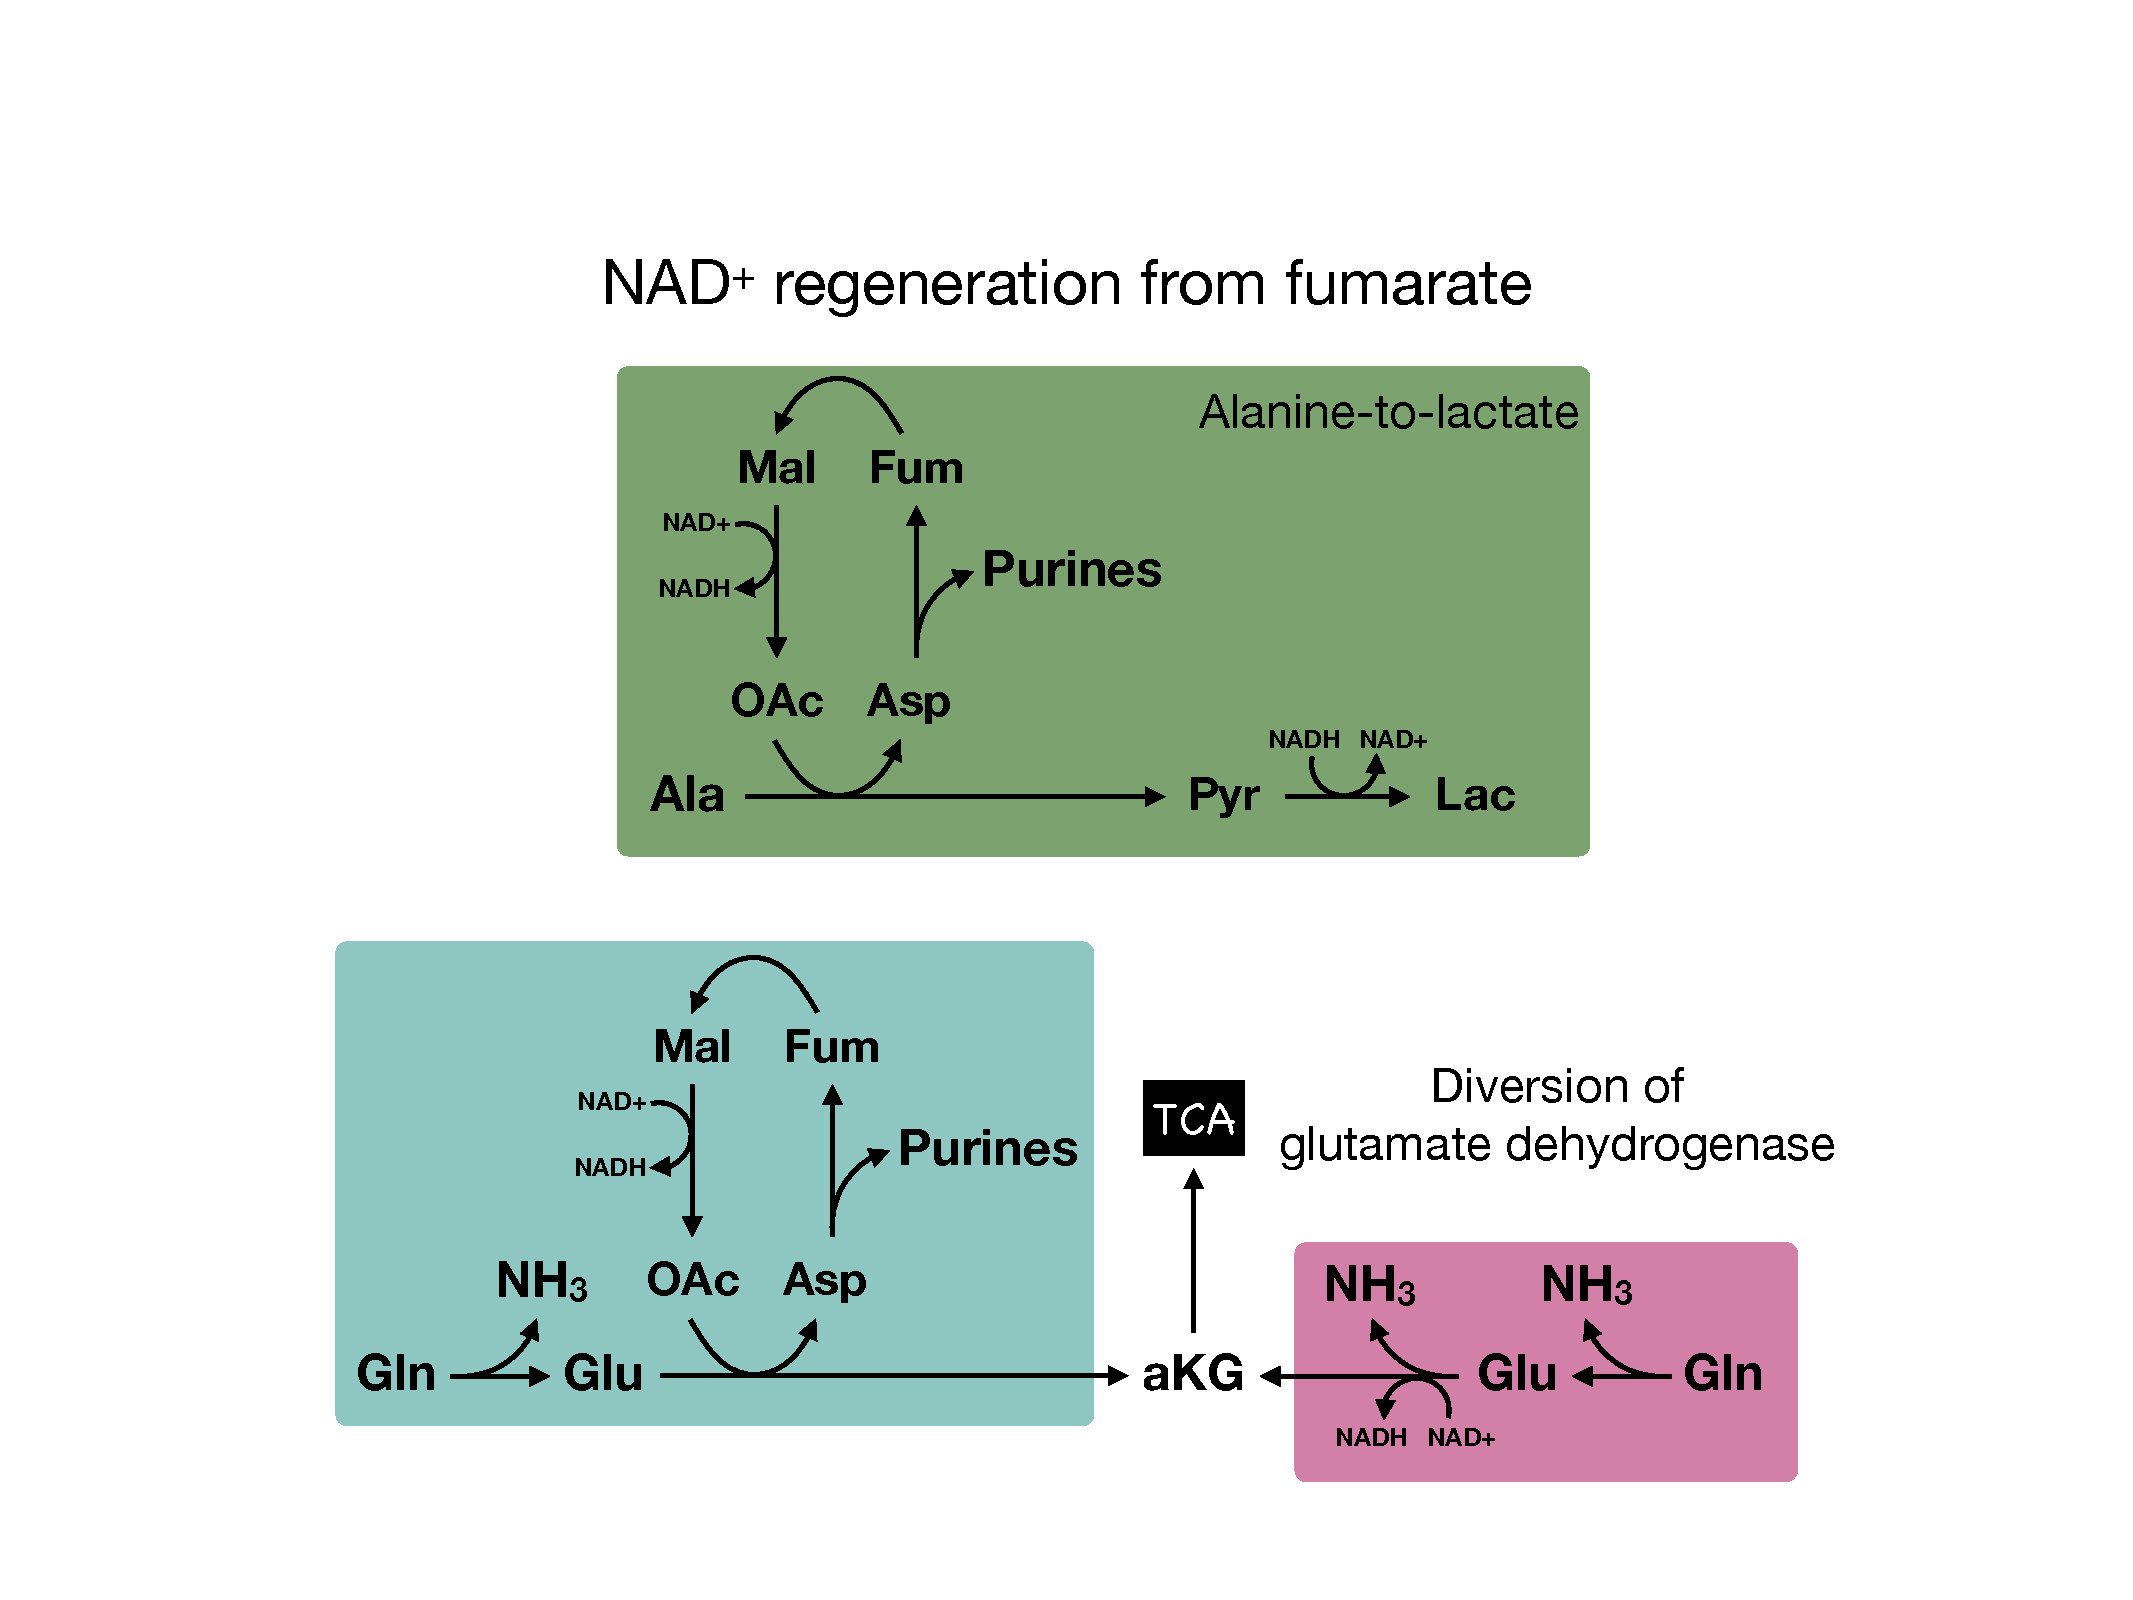
\includegraphics[width=0.7\textwidth]{figures/chap1/app/fumarate_NAD.pdf}
    \caption[Fumarate regeneration to aspartate.]{
    Fumarate regeneration to aspartate from via. either alanine-to-lactate conversion or diversion of \NAD{} consumption by glutamate dehydrogenase.
    }
    \label{fig:app_ch1:fumarate_NAD}
\end{figure}
